One of the scenarios where the proposed approach fails is when a person is moving in the same direction as user. The pedestrian detector detects the person and so the image is passed through the proposed multi-stream network. The network outputs an inaccurate estimate of time-to-collision as shown in Figure \ref{fig:misprediction}.

\begin{figure}[ht]
    \centering
        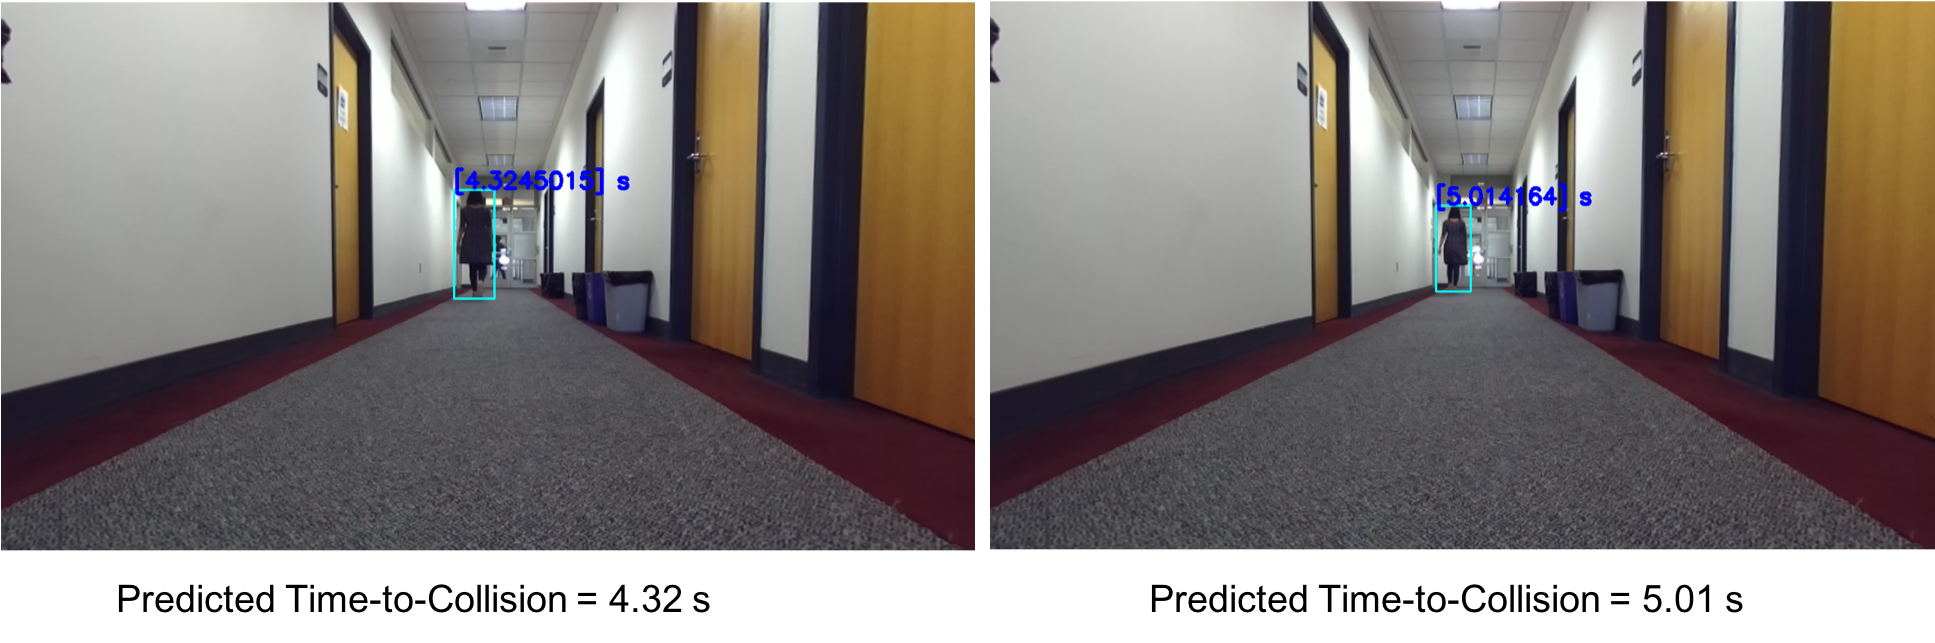
\includegraphics[height=5.0cm,width=\textwidth]{figs/mispredictions.png}
    \caption{Inaccurate estimate of time-to-collision when a person is moving away from the assistive suitcase}\label{fig:misprediction}
\end{figure}

Instead of passing the image first through the pedestrian detector, if we can instead pass it through a binary classifier trained to classify if there is going to be a collision within the chosen time bound (here, 6 seconds) or not. If positive, we can then pass it through the regressor network as proposed in this work to estimate the exact time-to-collision. OpenPose \cite{OpenPose}, a realtime approach to detect the 2D pose of multiple people in an image including foot, torso, arms and face keypoints can be leveraged to replace the object detection backbone, i.e, VGG-16 to enhance the prediction performance. \\

The prediction time bound in this work is chosen to be 6 seconds arbitrarily. Depending on the application or the planner requirements, the time bound could be chosen accordingly. For a higher time bound, it would be challenging to learn the task within an acceptable error limit. The Table \ref{tab:different_horizons} reports how the error varies with prediction time horizon.
\begin{table}[h]
\caption {Mean Absolute Error in Predicted Time varying with the Prediction Time Horizon} \label{tab:different_horizons} 
\begin{tabular}{|P{0.45\textwidth}|P{0.45\textwidth}|} \hline
Prediction Time Horizon (in seconds)  &  Mean Absolute Error (in seconds) \\ \hline
5 &  0.565 \\ \hline 
6 &  0.753 \\ \hline %% From slides
7 & 0.903 \\ \hline
\end{tabular}
\end{table}

